%TOASK
%---------------------------------------------------------------------
%   documentclass
%---------------------------------------------------------------------
\documentclass[]{beamer}
% Class options include: notes, notesonly, handout, trans,
%                        hidesubsections, shadesubsections,
%                        inrow, blue, elcon-clr, grey, brown

%---------------------------------------------------------------------
%   packages
%---------------------------------------------------------------------
% Theme for beamer presentation.
\usepackage{beamerthemesplit}
% Other themes include: beamerthemebars, beamerthemelined,
%                       beamerthemetree, beamerthemetreebars
\usepackage[english]{babel}
\usepackage[enc=utf8]{hrlatex}
\usepackage[T1]{fontenc} %pekne makcene
\usepackage{lmodern} %spolu s T1 smooth font!
\usepackage{cite} %bibtex
\usepackage[numbers]{natbib}
\usepackage{color} %for \textcolor{declared-color}{text}
\usepackage{floatflt} %to have tables and text beside
\usepackage{colortbl} %for \rowcolor command
\usepackage{scalefnt} %for scale font
\usepackage{pifont} %for ticks (check symbols)
\usepackage{pgfplots}
\usepackage{xcolor} %for \colorlet
\usepackage{lipsum}
\usepackage{bm}
\usepackage{multirow}

\usepackage{tikz}
\usetikzlibrary{decorations.pathreplacing}
\usetikzlibrary{shapes,fit,calc,shadows,plotmarks}

\colorlet{city-clr}{green!70!black}
\colorlet{elcon-clr}{red}
\colorlet{event-clr}{blue}
\colorlet{waiting-clr}{olive}
\colorlet{cmt-clr}{gray}
\colorlet{oracle-clr}{orange!30}
\colorlet{cmt-clr}{gray}
\colorlet{oracle-clr}{orange!30}
\colorlet{algsec-clr}{black!50!red}

%---------------------------------------------------------------------
%   settings
%---------------------------------------------------------------------
\graphicspath{{./pics/}} %picture dir

\definecolor{tablehead}{RGB}{238,233,233} %nice smooth grey

\def\Tiny{ \font\Tinyfont = cmr10 at 3pt \relax  \Tinyfont}

\pgfrealjobname{presentation} % <-- NOTE: this needs to be the real document's basename
                        %     (else you'll only get an empty output file)

\newif\iffull
\fullfalse

\newif\iffinal % introduce a switch for draft vs. final document
\finaltrue % use this to compile the final document
\iffinal
  \newcommand{\inputTikZ}[1]{%
    \input{#1.tikz}%
  }
\else
  \newcommand{\inputTikZ}[1]{%
    \beginpgfgraphicnamed{#1-external}%
    \input{#1.tikz}%
    \endpgfgraphicnamed%
  }
\fi

%---------------------------------------------------------------------
%   environments
%---------------------------------------------------------------------
%\newcommand{\newblock}{}

\newcommand{\tick}{\ding{52}}
\newcommand{\cross}{\ding{55}}

%---------------------------------------------------------------------
%   theme
%---------------------------------------------------------------------
\usetheme{Darmstadt}
\usecolortheme{seahorse}

%---------------------------------------------------------------------
%   data
%---------------------------------------------------------------------
\title{\textbf{Underlying shortest paths in timetables}}
\subtitle{Podkladové najkratšie cesty v cestovných poriadkoch}
\author{\textbf{František Hajnovič}}
\institute{FMFI UK}
\date{\today}

%---------------------------------------------------------------------
%   document
%---------------------------------------------------------------------
\begin{document}

	%---------------------------------------------------------------------
	%   Title page
	%---------------------------------------------------------------------
	{
    \setbeamertemplate{background canvas}{
        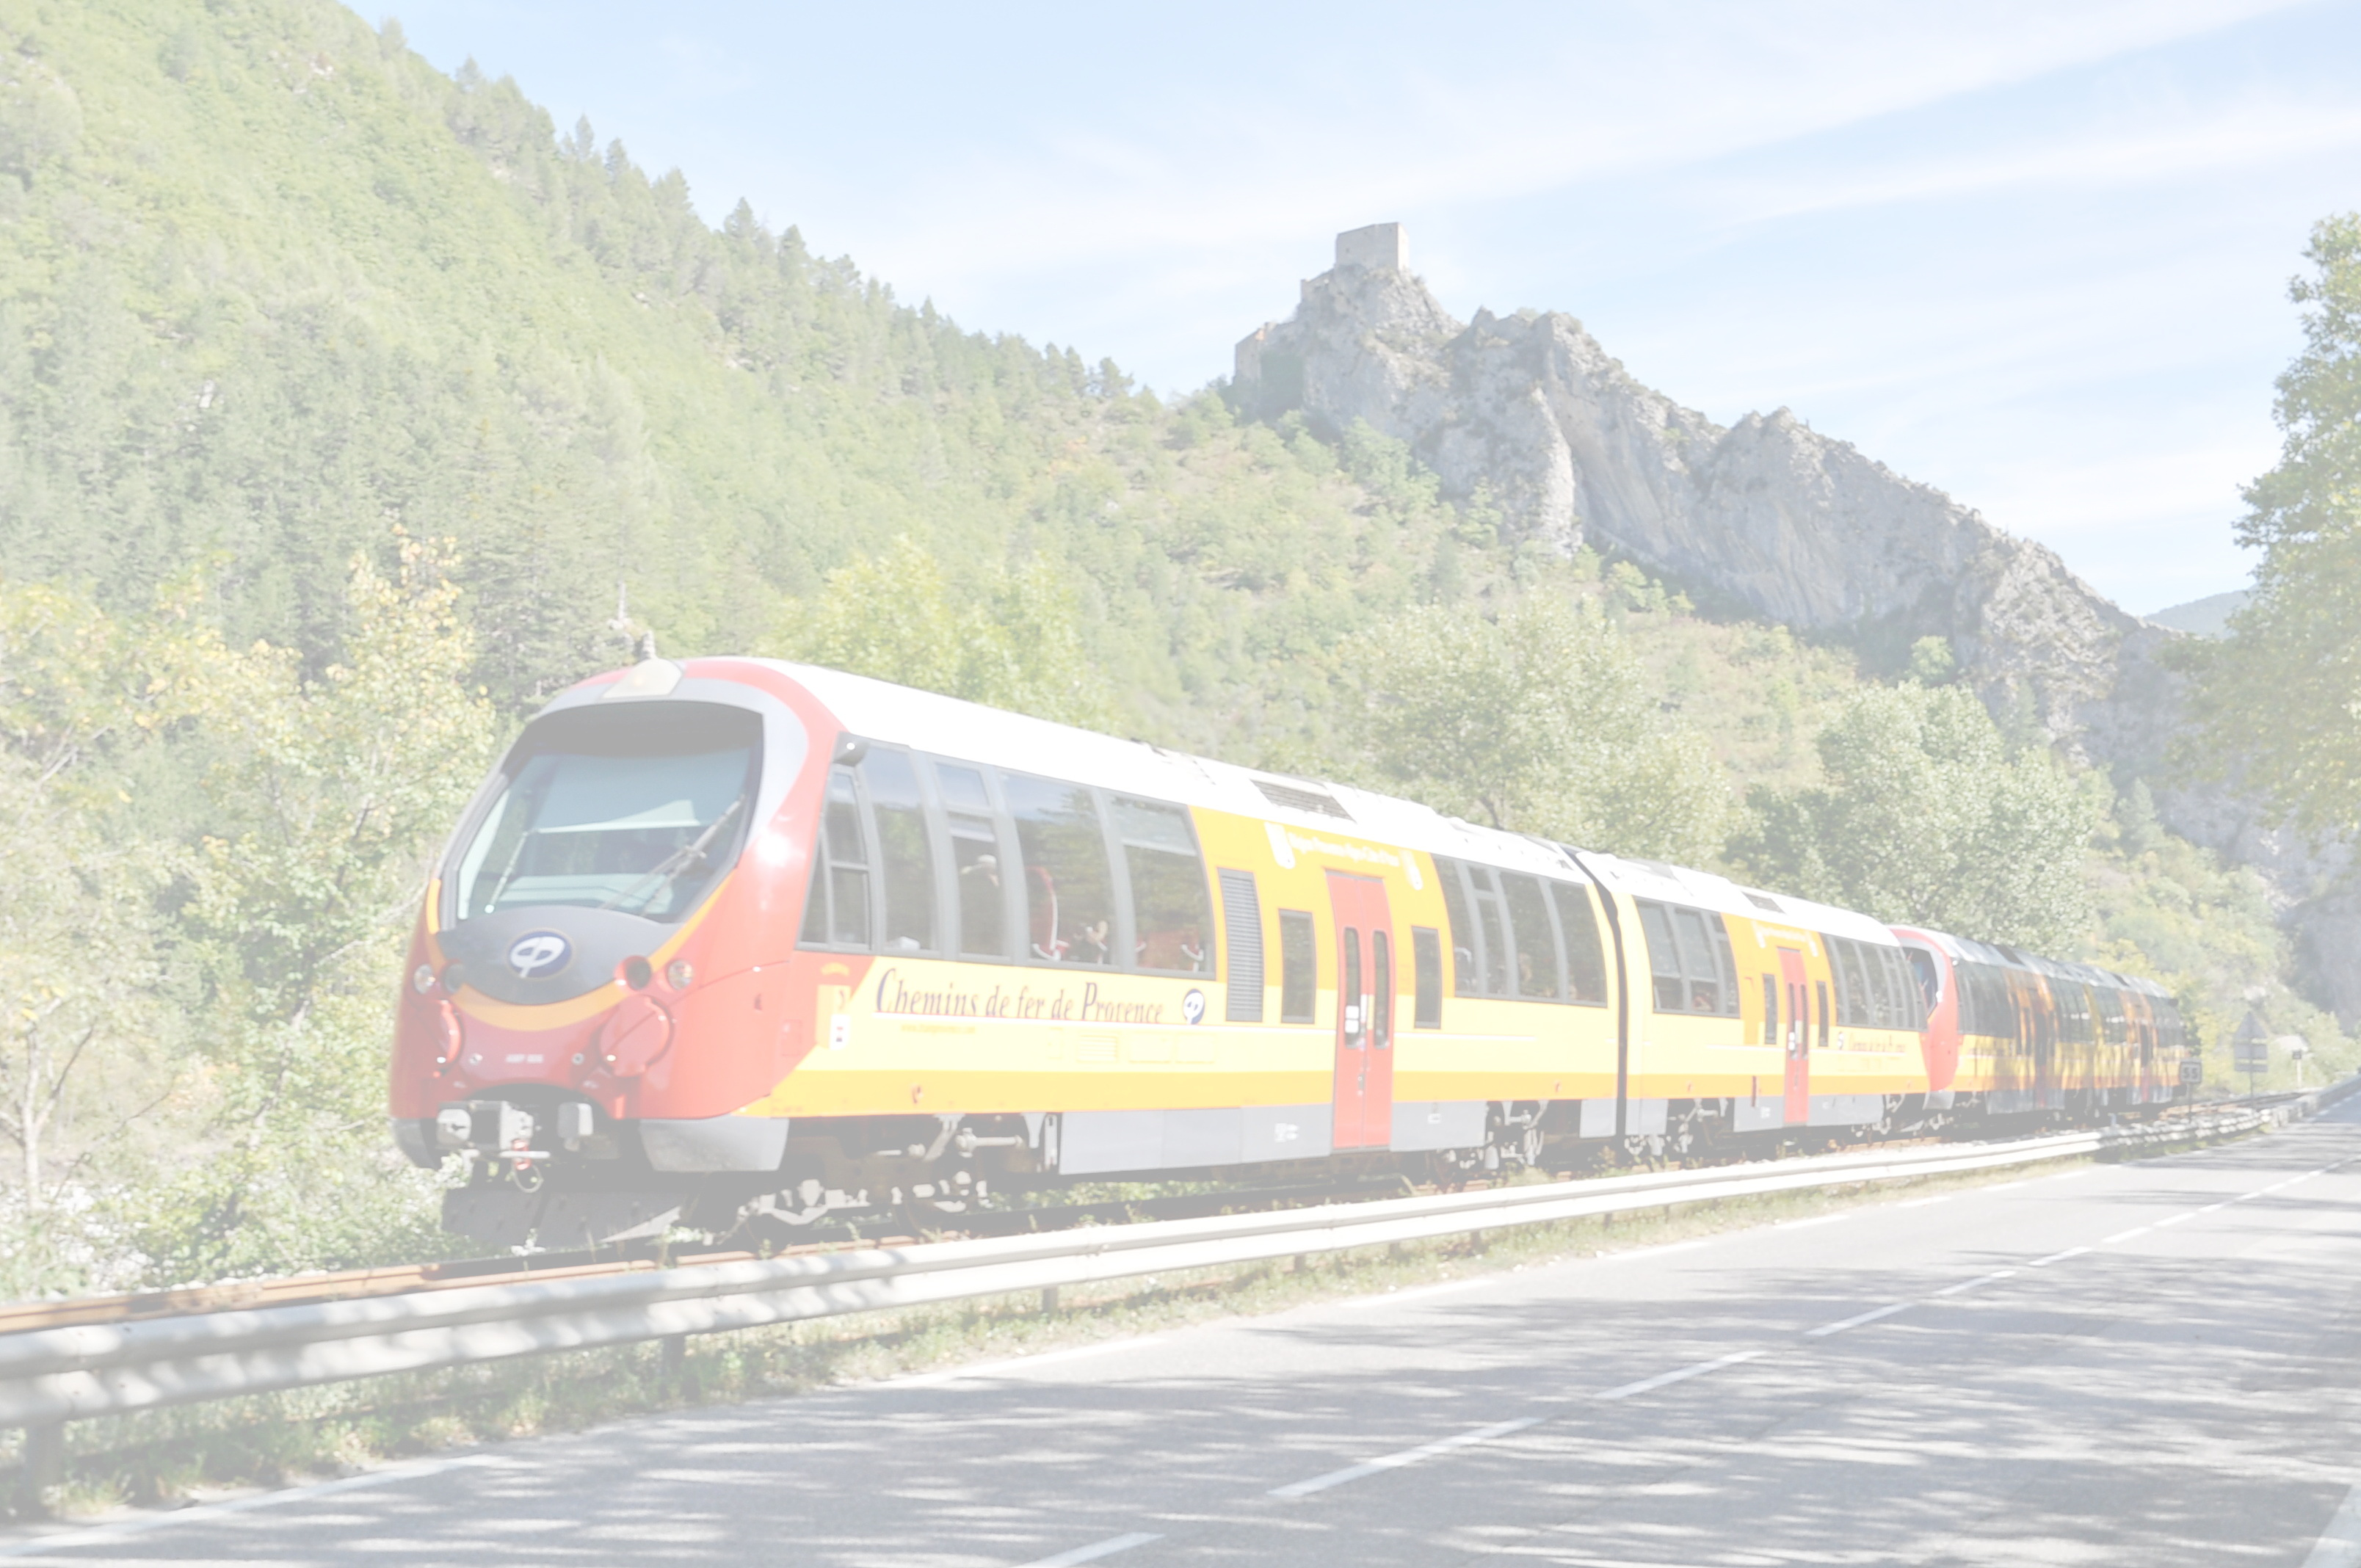
\includegraphics[height=\paperheight]{train.jpg}
    }
    \begin{frame}
        \titlepage
        \begin{center}
            Supervisor: \textit{doc. RNDr.} Rastislav Královič \textit{PhD.}
        \end{center}
    \end{frame}
    }

	%---------------------------------------------------------------------
	%   Content
	%---------------------------------------------------------------------
    \begin{frame}
        \frametitle{Content}
        \tableofcontents
    \end{frame}

	%---------------------------------------------------------------------
	%   Introduction
	%---------------------------------------------------------------------
    \setbeamercolor{frametitle}{fg=elcon-clr!80!black}
    \section{Introduction}
    \begin{frame}
        \frametitle{Introduction}
        \begin{center}
            \textcolor{elcon-clr!80!black}{\textbf{Introduction}}
        \end{center}
    \end{frame}
    \setbeamercolor{frametitle}{fg=black!70}

		%---------------------------------------------------------------------
		%   What is it about?
		%---------------------------------------------------------------------
	    \begin{frame}
	        \frametitle{What is it about?}
	        \begin{itemize}
	        	\small
	            \item Given a timetable, we query for \textbf{optimal connection} (OC): $\bm{(a, t, b)} \rightarrow \bm{c_{(a, t, b)}^{*}}$
	        \end{itemize}
	        \vspace{-0.5cm}
	        \begin{figure}[h!]
				\scriptsize
                \begin{center}
					\inputTikZ{./tikzpics/connection}
                \end{center}
            \end{figure}
            \vspace{-0.5cm}	
            \begin{itemize}
            	\small
            	\item<2> Motivation: large-scale timetable search engines (\emph{cp.sk, imhd.sk}...)
				\item<2> Approach: (distance) oracle-based approach~\cite{apxdo05} - pre-computation
			\end{itemize}
			\vspace{-0.5cm}
			\uncover<2>{\begin{figure}[h!]
				\scriptsize
                \begin{center}
					\inputTikZ{./tikzpics/oracle}
                \end{center}
			\end{figure}}
	    \end{frame}
	    
	    %---------------------------------------------------------------------
        %   TT and UG graph
        %---------------------------------------------------------------------
        \begin{frame}
            \frametitle{Timetable and underlying graph}        
	        \begin{columns}[c]
            \column{2.7in}
				\begin{table}{
	                \scriptsize
	                \begin{tabular}{c|c|c|c}
	                %legend
	                    \hline
	                    \rowcolor{tablehead}
	                    \multicolumn{2}{>{\columncolor{tablehead}}c|}{\textbf{Place}} & \multicolumn{2}{>{\columncolor{tablehead}}c}{\textbf{Time}} \\
						\hline
	                    \rowcolor{tablehead}
	                    \textbf{From} & \textbf{To} & \textbf{Departure} & \textbf{Arrival} \\
	                %data
						\hline
	                    \textcolor{city-clr}{A} & \textcolor{city-clr}{B} & 10:00 & 10:45 \\
						\textcolor{city-clr}{B} & \textcolor{city-clr}{C} & 11:00 & 11:30 \\
						\textcolor{city-clr}{B} & \textcolor{city-clr}{C} & 11:30 & 12:10 \\
						\textcolor{city-clr}{B} & \textcolor{city-clr}{A} & 11:20 & 12:30 \\
						\textcolor{city-clr}{C} & \textcolor{city-clr}{A} & 11:45 & 12:15 \\
					\end{tabular}}
					\caption{\textbf{Timetable} - a set of \textbf{elementary connections} (between pairs of \textbf{\textcolor{city-clr}{cities}}).}
	            	\normalsize
				\end{table}
            \column{2.3in}
            	\begin{figure}[h!]
					\scriptsize
	                \begin{center}
						\inputTikZ{./tikzpics/ug}
	                \end{center}
                    \caption{\textbf{Underlying graph}.}
                \end{figure}
			\end{columns}
			\begin{itemize}
				\item<2> Goals:
				\begin{itemize}
	                \item<2> Devise methods to tackle EA/OC problem
		            \item<2> Analyse properties of real-world timetables
	            \end{itemize}			
			\end{itemize}
		\end{frame}
		
	%---------------------------------------------------------------------
	%   Contribution 
	%---------------------------------------------------------------------
    \setbeamercolor{frametitle}{fg=elcon-clr!80!black}
    \section{Contribution}
    \begin{frame}
        \frametitle{Contribution}
        \begin{center}
            \textcolor{elcon-clr!80!black}{\textbf{Contribution}}
        \end{center}
    \end{frame}
    \setbeamercolor{frametitle}{fg=black!70}

	    %---------------------------------------------------------------------
        %   Idea
        %---------------------------------------------------------------------
        \subsection{Underlying shortest paths}
        \begin{frame}
            \frametitle{Idea}
			\begin{itemize}
                \item \textit{``Usually we go through the same sequence of cities''}
            \end{itemize}
            \vspace{0.5cm}
            \begin{columns}[c]
            \column{2.7in}
            	\vspace{-1cm}
	            \begin{figure}[h]
					\scriptsize
	                \begin{center}
	                    \inputTikZ{./tikzpics/pathfunc}
	                \end{center}
	            \end{figure}
	            \vspace{-0.7cm}
	            \begin{itemize}
	            	\small
	            	\item $p$ is \textbf{USP} $\iff$ $\exists t: path(c_{(a, t, b)}^{*}) = p$
	            	\item we have USP $p$: $expand(p)$ $\rightarrow$ $c_{(a, t, b)}^{*}$
	            	\item<2-> \textbf{Overtaking}~\cite{timetablemodelsalgs07} causes problems, but can be easily removed
	            \end{itemize}
	        \column{2.3in}
		        \vspace{-0.5cm}
	        	\begin{figure}[h!]
	                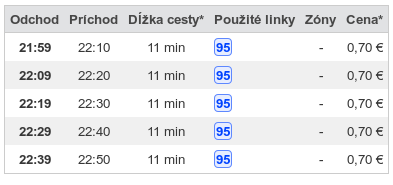
\includegraphics[height=0.9in]{redundancy.png}
	            \end{figure}
	            \uncover<2->{
	            	\vspace{-0.5cm}
	            	\begin{table}{
	                \tiny
	                \begin{tabular}{c|c}
	                %legend
	                    \hline
	                    \rowcolor{tablehead}
	                    \textbf{Name} & \textbf{Overtaken edges (\%)} \\
	                %data
						\hline
						\textit{air01} & 1\% \\
						\textit{cpsk} & 2\% \\
						\textit{gb-coach} & 1\% \\
						\textit{gb-train} & 0\% \\
						\textit{montr} & 1\% \\
						\textit{sncf} & 1\% \\
						\textit{sncf-ter} & 1\% \\
						\textit{sncf-inter} & 6\% \\
						\textit{zsr} & 0\% \\
					\end{tabular}}
	            	\normalsize
				\end{table}}
			\end{columns}
        \end{frame}
        
        %---------------------------------------------------------------------
        %   USP-OR
        %---------------------------------------------------------------------
        \subsection{USP-OR}
        \begin{frame}
            \frametitle{\textit{USP-OR}}
            \begin{columns}[c]
            \column{2.4in}
				\begin{itemize}
					\small
					\item<1-> Pre-compute \textit{all conn.} - space $\mathcal{O}(h \; n^{2} \gamma)$
					\begin{itemize}
						\item $\bm{\gamma}$ - the average OC size
	                	\item $\bm{h}$ - height
	                \end{itemize}
	                \item<2-> Pre-compute \textit{all USPs} - space $\mathcal{O}(\tau \; n^{2} \gamma)$
	                \begin{itemize}
	                	\item $\bm{\tau(x, y)}$ - \# of USPs between $x$ and $y$
	                \end{itemize}
	                \item<2-> $\bm{\delta}$ - the density of UG
				\end{itemize}
	        \column{2.6in}
	        	\uncover<2->{\begin{table}{
	                \scriptsize
	                \begin{tabular}{c|c|c|c|c}
	                %legend
	                    \hline
	                    \rowcolor{tablehead}
	                    \textbf{Name} & \textbf{$\bm{\tau}$} & \textbf{$\bm{\gamma}$} & \textbf{$\bm{\delta}$} & \textbf{$\bm{h}$} \\
	                %data
						\hline
						\textit{air01} & 7.5 & 2.1 & 32.9 & 112.7 \\
						\textit{cpsk} & 12.1 & 15.9 & 3.9 & 50.7 \\
						\textit{gb-coach} & 5.3 & 5.3 & 5.6 & 48 \\
						\textit{gb-train} & 10.3 & 7.6 & 5.7 & 129.6 \\
						\textit{montr} & 5.1 & 21.0 & 1.9 & 35.0 \\
						\textit{sncf} & 5.6 & 8.6 & 3.4 & 42.4 \\
						\textit{sncf-inter} & 2.6 & 13.4 & 1.1 & 20.8 \\
						\textit{sncf-ter} & 5.6 & 12.7 & 3.3 & 34.0 \\
						\textit{zsr} & 3.7 & 13.5 & 2.7 & 21.6 \\
					\end{tabular}}
					\caption{\footnotesize Daily, 200 station timetable subsets.}
	            	\normalsize
				\end{table}}
	        \end{columns}
	        \makebox[\linewidth]{\parbox{12cm}{
	        \uncover<2->{\begin{table}[h!]
	        	\scriptsize
				\centering
				\begin{tabular}{l|c|c|c|c}
				%legend
					\cellcolor{oracle-clr} \textit{\textbf{USP-OR}} & \cellcolor{oracle-clr} $\bm{prep}$ & \cellcolor{oracle-clr} $\bm{size}$ & \cellcolor{oracle-clr} $\bm{qtime}$ & \cellcolor{oracle-clr} $\bm{stretch}$ \\
				%data
					\hline
					\cellcolor{oracle-clr} \textbf{guaranteed} & $\mathcal{O}(hn^{2} (\log n + \delta))$ & $\mathcal{O}(\tau n^{2} \gamma)$ & avg. $\mathcal{O}(\tau \gamma)$ & $1$ \\
					\cellcolor{oracle-clr} \textbf{$\bm{\tau}$ const., $\bm{\gamma \leq \sqrt{n}}$, $\bm{\delta \leq \log n}$} & $\mathcal{O}(hn^{2} \log n)$ & $\mathcal{O}(n^{2.5})$ & avg. $\mathcal{O}(\sqrt{n})$ & $1$ \\
				\end{tabular}
			\end{table}}
			}}
        \end{frame}
        
        %---------------------------------------------------------------------
        %   USP-OR - grafy
        %---------------------------------------------------------------------
        \begin{frame}
            \frametitle{\textit{USP-OR} - $\tau$ evolution}
            \begin{columns}[c]
            \column{2.4in}
				\begin{figure}[h]
					\scriptsize
	                \begin{center}
	                    \only<1>{\inputTikZ{./tikzpics/plot_usp_sncf_trange}}
	                    \only<2->{\inputTikZ{./tikzpics/plot_uspseg_sncf_trange}}
	                \end{center}
	                \caption{\footnotesize Changing of $\tau$ with increased time range in \textit{gb-sncf-200} dataset. \only<2->{\textbf{Segmentation} of the timetable to days.}}
	            \end{figure}
	        \column{2.4in}
	        	\uncover<3->{\begin{figure}[h]
					\scriptsize
	                \begin{center}
	                    \inputTikZ{./tikzpics/plot_usp_gbcoach_size}
	                \end{center}
	                \caption{\footnotesize Changing of $\tau$ with increased \# of stations in \textit{gb-coach} dataset.}
	            \end{figure}}
	        \end{columns}
			\begin{itemize}
				\item<4-> Space $\mathcal{O}(n^{2.5})$ too big anyway...
			\end{itemize}
        \end{frame}
        
        %---------------------------------------------------------------------
        %   USP-OR-A
        %---------------------------------------------------------------------
        \subsection{USP-OR-A}
        \begin{frame}
            \frametitle{\textit{USP-OR-A}}
		    \footnotesize
			\begin{itemize}
				\item Pre-compute USPs only among \textit{some} cities in UG: $\bm{(r_{1}, r_{2}, r_{3})}$ \textbf{access node set} $\mathcal{A}$
				\begin{itemize}
					\footnotesize
					\item Small size: $|\mathcal{A}| \leq r_{1} \cdot \sqrt{n}$
					\item Small node neighbourhoods: $avg \; (|neigh(x)|)^{2} \leq r_{2} \cdot n$
					\item Few local access nodes: $avg (|lan_{\mathcal{A}}(x)|)^{2} \leq r_{3}$
				\end{itemize}
	        \end{itemize}
	        \vspace{-0.35cm}
	        \makebox[\linewidth]{\parbox{12cm}{\begin{figure}[h]
				\scriptsize
                \begin{center}
					\inputTikZ{./tikzpics/uspora}
                \end{center}
            \end{figure}
            }}
        \end{frame} 
        
		%---------------------------------------------------------------------
        %   USP-OR-A and ANs
        %---------------------------------------------------------------------        
        \begin{frame}
            \frametitle{\textit{USP-OR-A} and access nodes}
            \vspace{-0.2cm}
		    \makebox[\linewidth]{\parbox{12cm}{\begin{table}[h!]
				\centering
				\tiny
				\begin{tabular}{l|c|c}
				%legend
					\cellcolor{oracle-clr} \textit{\textbf{USP-OR-A}} & 
					\cellcolor{oracle-clr} \textbf{guaranteed} & 
					\cellcolor{oracle-clr} \textbf{$\bm{\tau, r_{1}, r_{2}, r_{3}}$ const., $\bm{\gamma \leq \sqrt{n}}$, $\bm{\delta \leq \log n}$} \\
				%data
					\hline
					\cellcolor{oracle-clr} $\bm{prep}$ & $\mathcal{O}(f(n) + (r_{1} + r_{2}) (\delta + \log n) h n^{1.5})$ & $\mathcal{O}(f(n) + h n^{1.5} \log n)$ \\
					\cellcolor{oracle-clr} $\bm{size}$ & $\mathcal{O}(r_{2} n^{1.5} + r_{1}^{2} \tau_{\mathcal{A}} \gamma_{\mathcal{A}} n)$ & $\mathcal{O}(n^{1.5})$ \\
					\cellcolor{oracle-clr} $\bm{qtime}$ & avg. $\mathcal{O}(r_{2} r_{3} \sqrt{n} (\log (r_{2}n) + \delta) + r_{3} \tau_{\mathcal{A}} \gamma_{\mathcal{A}})$ & avg. $\mathcal{O}(\sqrt{n} \log n)$ \\
					\cellcolor{oracle-clr} $\bm{stretch}$ & $1$ & $1$ \\
				\end{tabular}
			\end{table}
			}}
			\vspace{-0.5cm}
			\begin{itemize}
				\small
				\item<2-> Minimize $|\mathcal{A}|$ s.t. $\forall x: |neigh_{\mathcal{A}}(x)| \leq \sqrt{n}$ $\rightarrow$ NP-complete
			\end{itemize}
			\vspace{-0.2cm}
			\begin{columns}[c]
            \column{2.8in}
	            \begin{itemize}
					\small
					\item<3-> Choose ANs based on degree/betweenness centrality
				\end{itemize}
				\vspace{-0.2cm}
            	\uncover<3->{\begin{figure}[h]
					\scriptsize
	                \begin{center}
	                    \inputTikZ{./tikzpics/plot_hdeg_sncf_size}
	                \end{center}
	                \vspace{-0.3cm}
	                \caption{\scriptsize \textit{sncf}, $r_{2} \leq 1$.}
	            \end{figure}}
	        \column{2.4in}
	        	\begin{itemize}
	        	\small
            		\item<4-> Select AN that locally separates many vertices
         	   \end{itemize}
         	   \vspace{-0.5cm}
         	   \uncover<4->{\begin{figure}[h]
					\scriptsize
	                \begin{center}
						\inputTikZ{./tikzpics/locsep}
	                \end{center}
	            \end{figure}}
	        \end{columns}
        \end{frame} 
        
        %---------------------------------------------------------------------
        %   Locsep
        %---------------------------------------------------------------------
        \begin{frame}
            \frametitle{\textit{Locsep}}
            \begin{itemize}
            	\item Select AN that locally separates many vertices
            \end{itemize}
            \begin{columns}[c]
            \column{2.5in}
	            \begin{figure}[h]
					\scriptsize
	                \begin{center}
	                    \inputTikZ{./tikzpics/plot_locsep_sncf_size}
	                \end{center}
	                \vspace{-0.3cm}
	                \caption{\scriptsize \textit{sncf}, $r_{2} \leq 1$.}
	            \end{figure}
	        \column{2.5in}
	        	\begin{figure}[h]
					\scriptsize
	                \begin{center}
	                    \inputTikZ{./tikzpics/plot_locsep_gbcoach_size}
	                \end{center}
	                \vspace{-0.3cm}
	                \caption{\scriptsize \textit{gb-coach}, $r_{2} \leq 1$.}
	            \end{figure}
	        \end{columns}

        \end{frame}
        
		%---------------------------------------------------------------------
        %   Performance
        %---------------------------------------------------------------------
        \subsection{Performance}
        \begin{frame}
            \frametitle{Performance}
            \begin{itemize}
            	\item Time-dependent Dijkstra's algorithm with Fibonacci heap priority queue $\mathcal{O}(m + n \log n)$
            \end{itemize}
			\begin{columns}[c]
            \column{2.4in}
				\begin{figure}[h]
					\scriptsize
	                \begin{center}
	                    \inputTikZ{./tikzpics/plot_usporall_sncf_size}
	                \end{center}
	                \caption{\footnotesize query time, \textit{sncf}}
	            \end{figure}
	        \column{2.4in}
	        	\begin{figure}[h]
					\scriptsize
	                \begin{center}
	                    \inputTikZ{./tikzpics/plot_usporall_gbcoach_size}
	                \end{center}
	                \caption{\footnotesize query time, \textit{gb-coach}}
	            \end{figure}
	        \end{columns}
        \end{frame}
        
		%---------------------------------------------------------------------
        %   Performance
        %---------------------------------------------------------------------        
        
        \begin{frame}
            \frametitle{Performance}
			\begin{table}[h!]
		        \centering
		        \tiny
				\begin{tabular}{c|c|c|c|c|c|c|c}
				%legend
					\rowcolor{tablehead}
					 & \textbf{Dataset} & \multicolumn{2}{>{\columncolor{tablehead}}c|}{\textit{sncf}} & \multicolumn{2}{>{\columncolor{tablehead}}c|}{\textit{gb-coach}} & \multicolumn{2}{>{\columncolor{tablehead}}c}{\textit{gb-train}} \\ \cline{1-8}
					\rowcolor{tablehead}
					 & \textbf{Time range} & (1 day) & (1 week) & (1 day) & (1 week) & (1 day) & (1 week) \\			
				%data
					\hline
					\rowcolor{tablehead} & $\bm{n}$ & 1000 & 700 & 1000 & 700 & 700 & 500 \\ cline{2-8}
					\cellcolor{tablehead} & \cellcolor{tablehead} \textbf{Speed-up} & 0 & 0 & 0 & 0 & 0 & 0 \\
					\multirow{-3}{*}{\textit{USP-OR}} \cellcolor{tablehead} & \cellcolor{tablehead} \textbf{Size-up} & 0 & 0 & 0 & 0 & 0 & 0 \\
					\hline
					\rowcolor{tablehead}  & $\bm{n}$ & 2608 & 2646 & 2406 & 2448 & 2550 & 2555 \\ \cline{2-8}
					\cellcolor{tablehead} & \cellcolor{tablehead} \textbf{Speed-up} & 0 & 6.3 & 0 & 8.8 & 0 & 2.8 \\
					\multirow{-3}{*}{\textit{USP-OR-A}} \cellcolor{tablehead} & \cellcolor{tablehead} \textbf{Size-up} & 0 & 7.8 & 0 & 10.4 & 0 & 5.2 \\
				\end{tabular}
			\end{table}
			\vspace{-0.5cm}
			\begin{columns}[c]
            \column{2.4in}
				\begin{figure}[h]
					\scriptsize
	                \begin{center}
	                    \inputTikZ{./tikzpics/plot_uspors_sncf_size}
	                \end{center}
	                \caption{\footnotesize \textit{USP-OR} oracle size, \textit{sncf}}
	            \end{figure}
	        \column{2.4in}
				\begin{figure}[h]
					\scriptsize
	                \begin{center}
	                    \inputTikZ{./tikzpics/plot_usporas_sncf_size}
	                \end{center}
	                \caption{\footnotesize \textit{USP-OR-A} oracle size, \textit{sncf}}
	            \end{figure}
	        \end{columns}
        \end{frame}   
        
        %---------------------------------------------------------------------
        %   Existing methods
        %---------------------------------------------------------------------
        \begin{frame}
            \frametitle{Existing methods}
			\begin{itemize}
				\item \textbf{Time-dependent SHARC} \cite{sharc08}, \textbf{Time-dependent CH} \cite{timedepch09}
				\begin{itemize}
					\item Speed-ups of about 26 / 1500, respectively (EA only)
					\item Meant for time-dependent routing in road networks
				\end{itemize}
				\item \textbf{Engineering time-expanded graphs...} \cite{engtimeexp09}
		        \begin{itemize}
					\item Max speed-up of 56 (Railways with 30000 stations!)
					\item Remodelling unimportant stations in TE graphs
				\end{itemize}
				\item<2-> Theory vs. practice difference
				\begin{itemize}
					\item More complicated (transfers, cost of travel...)
					\item Focus on one given dataset
				\end{itemize}
			\end{itemize}
        \end{frame}            
    
    %---------------------------------------------------------------------
	%   Conclusion
	%---------------------------------------------------------------------
    \setbeamercolor{frametitle}{fg=elcon-clr!80!black}
    \section{Conclusion}
    \begin{frame}
        \frametitle{Conclusion}
        \begin{center}
            \textcolor{elcon-clr!80!black}{\textbf{Conclusion}}
        \end{center}
    \end{frame}
    \setbeamercolor{frametitle}{fg=black!70}
    
    	%---------------------------------------------------------------------
        %   Conclusion
        %---------------------------------------------------------------------
        \begin{frame}
            \frametitle{Conclusion}
            \begin{itemize}
				\item \textbf{Application} created to carry out \textbf{analysis} of real-world timetables:
				\begin{itemize}
					\item Degrees, connectivity, BC, highway dimension, overtaking, USPs...
					\item Running \& evaluating tests of oracles
				\end{itemize}
				\item<2-> Trying out \textbf{novel approaches} to find optimal connections in timetables
				\begin{itemize}
					\item \textit{USP-OR}: Exact and very quick answers (speed-up $\approx$ 60) but high space
					\item \textit{USP-OR-A}: Exact and quick answers (speed-up $\approx$ 6) less space-consuming
					\item \textit{NN}: Problem too challenging for NN/try different types of network
				\end{itemize}
			\end{itemize}
        \end{frame}
        
%---------------------------------------------------------------------
%   Bibliography
%---------------------------------------------------------------------
    \begin{frame}[allowframebreaks]
        \frametitle{Bibliography}
        \tiny
        \bibliographystyle{is-alpha}
        \bibliography{../bibl}
        %compile latex, bibtex, latex, latex
    \end{frame}

%---------------------------------------------------------------------
%   Thanks for the attention
%---------------------------------------------------------------------
	{
    \setbeamertemplate{background canvas}{
        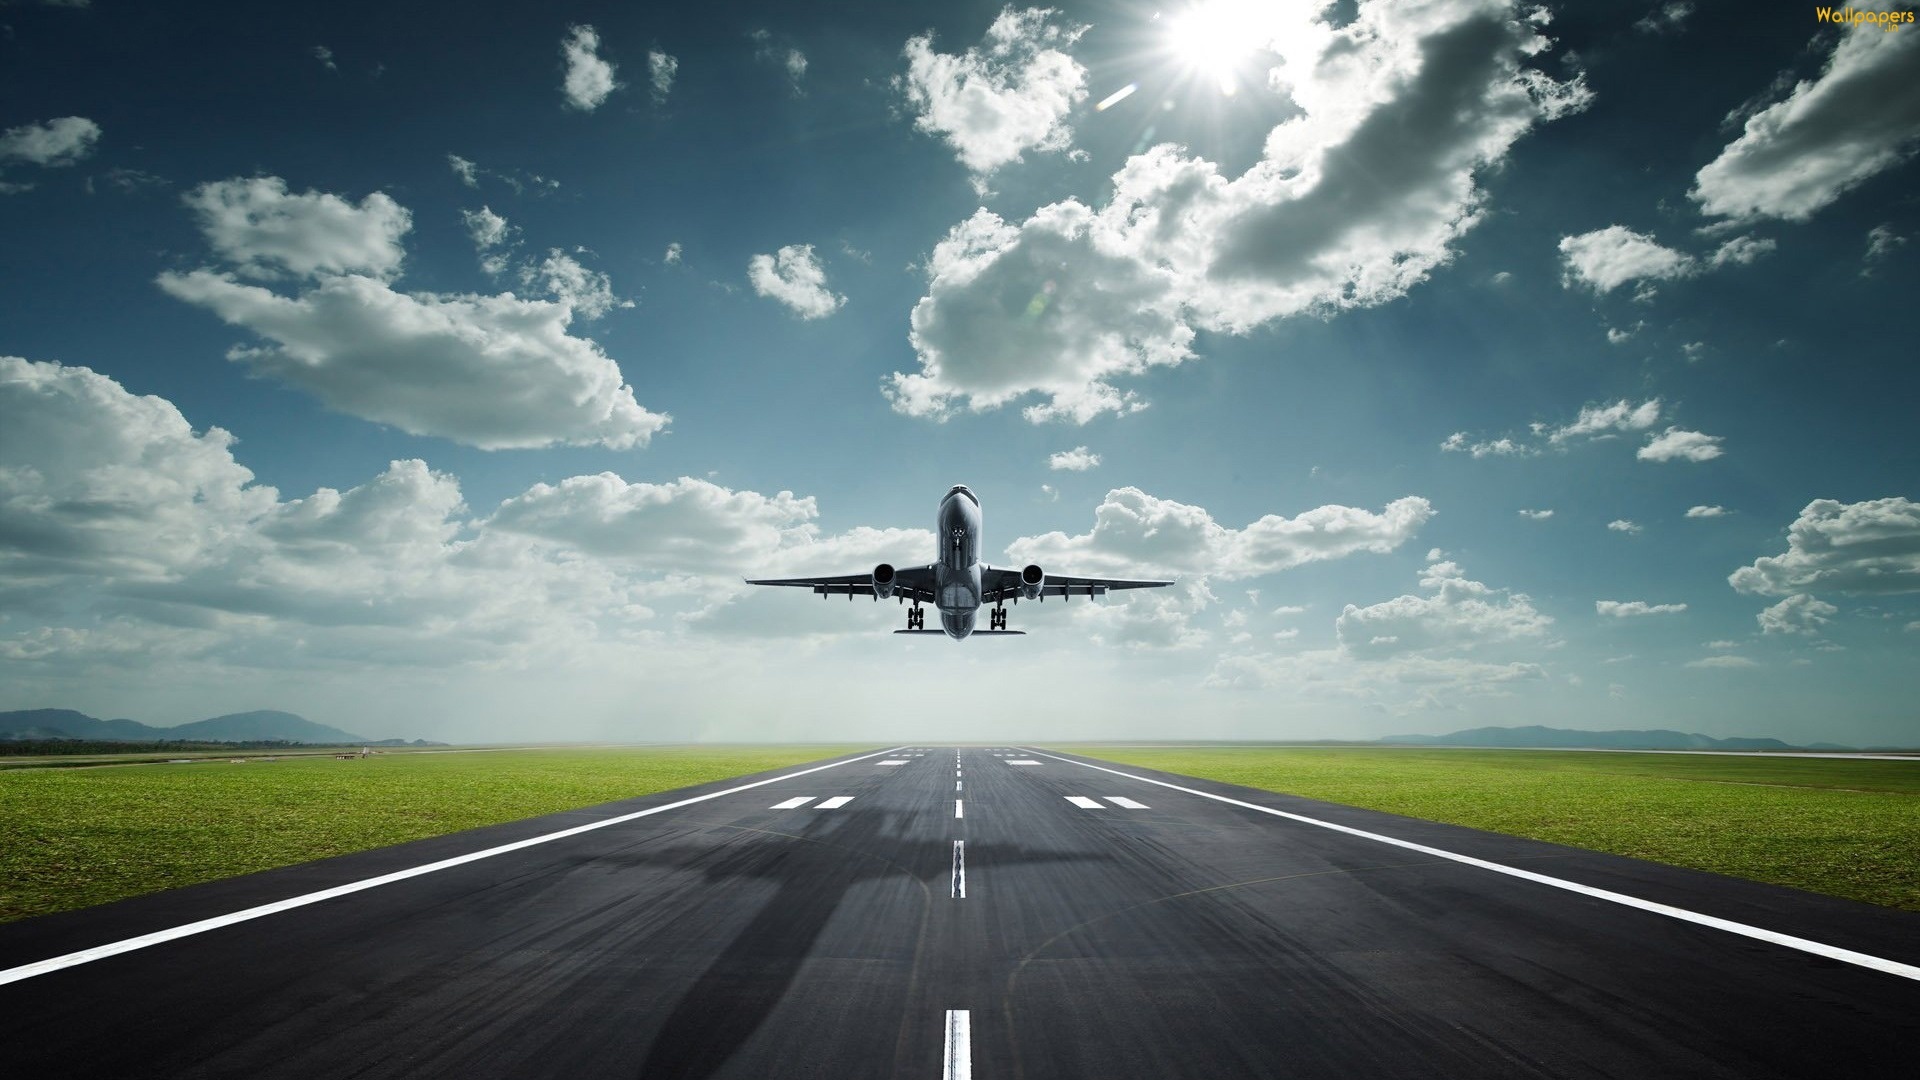
\includegraphics[height=\paperheight]{takeoff.jpg}
    }
    \begin{frame}
        \frametitle{Thank you for the attention}
        \begin{center}
        	\vskip 2cm
            \textbf{Thank you for the attention}
        \end{center}
    \end{frame}
    }

\end{document}
